\documentclass{article}
\usepackage{amsmath,amscd,amsbsy,amssymb,latexsym,url,bm,amsthm}
\usepackage{epsfig,graphicx,subfigure}
\usepackage{enumitem,balance,mathtools}
\usepackage{wrapfig}
\usepackage{mathrsfs, euscript}
\usepackage{hyperref}
\usepackage{listings}
\usepackage[ruled,lined,boxed,linesnumbered]{algorithm2e}
\usepackage{amsthm}
\usepackage{tikz}

\newtheorem*{solution}{Solution}


\renewcommand{\thefootnote}{\fnsymbol{footnote}}
\newcommand{\postscript}[2]
    {\setlength{\epsfxsize}{#2\hsize}
    \centerline{\epsfbox{#1}}}
\renewcommand{\baselinestretch}{1.0}



\title{EI338 Lab Report Chapter2}
\author{Bao Xiaoyi 517030910306}
\date{October 16,  2019}

\begin{document}

\maketitle

\section{Environment}
\begin{itemize}
    \item VirtualBox 5.2.18
    \item Ubuntu 14.04 (64 bit) running on the virtual machine
\end{itemize}

\section{Assignment}
\begin{enumerate}
    \item Design a kernel module that creates a \texttt{/proc}  file named \texttt{/proc/jiffies} that reports the current value of \texttt{jiffies} when the \texttt{proc/jiffies} file is read, such as the command 
    \begin{verbatim}
        cat /proc/jiffies
    \end{verbatim}
    Be sure to remove \texttt{/proc/jiffies} when the module is removed.
    \item Design a kernel module that creates a \texttt{proc} file named \texttt{/proc/seconds} that reports the number of elapsed seconds since the kernel module was loaded. This ill involve using the value of \texttt{jiffies} as well as the \texttt{HZ} rate. When a user enters the command
    \begin{verbatim}
        cat /proc/seconds
    \end{verbatim}
    your kernel module will report the number of seconds that elapsed since the kernel module was first loaded. Be sure to remove the \texttt{/proc/seconds} when the module is removed.
\end{enumerate}

\newpage
\section{Decomposition and Analysis}
Here, we try to decompose the original tasks into smaller parts, and solve the sub problems one by one.
\begin{enumerate}
    \item Obtain the value of \texttt{HZ} and \texttt{jiffies} from certain module.
    \begin{solution}
    As noted in the textbook, the tick rate is the value \texttt{HZ} defined in \texttt{<asm/param.h>}. Also, the number of timer interrupts that have occured since the system was booted is stored as the global variable \texttt{jiffies} in \texttt{linux/jiffies.h}. Thus, we only need to import the two files, and make use of \texttt{HZ} and \texttt{jiffies} inside them.
    \end{solution}
    
    \item Consider the fact the variable \texttt{jiffies} changes its value every time we call it, we need to store its value when the module is first loaded.
    \begin{solution}
        we can store the original value of \texttt{jiffies} in a global variable. That is, it is at the same level as main{}. In this way, we can require it from any part of the code. 
    \end{solution}
    \item Figure out the relationship between elapsed time, frequency, and the number of timer interrupt.
    \begin{solution}.   
        Here, frequency means "ticks per second". We can represent the relationship among them with an equation:
        \begin{align*}
            t &= \frac {\Delta interrupt} {tick\_per\_ second} \\
            &= \frac {jiffies_2 - jiffirs_1} {HZ}
        \end{align*}
    \end{solution}
    \item Find a way to pass certain information from kernel to user.
    \begin{solution}
    The example file, \texttt{hello.c} may give us some hint on the topic. As is shown in the textbook, a buffer is used to store the message, and an extra integer variable contains the length of the string.
    \end{solution}
    \item Use terminal in Linux to check our solution.
    \begin{solution}
    We just need to compile the file, add it to the kernel, then interact with the command line.
    \end{solution}
\end{enumerate}

\newpage
\section{Details}
In this part, some codes are shown for better illustration.  We mainly show the difference between our file and the example file, \texttt{hello.c}

\begin{itemize}
    \item Two files that we include to deal with assignment1. 
    \begin{lstlisting}[language=C]
    
    /* jiffies.c*/
    #include <asm/uaccess.h>
    #include <linux/jiffies.h>
    
    /* in function proc_read */
    rv = sprintf(buffer, 
    "The current value of jiffies is : %lu \n", jiffies);
    
    /* the length, together with the length, 
    is passed to the user */
    copy_to_user(usr_buf, buffer, rv);
    \end{lstlisting}
    
    \item We made some further modification to the original file to satisfy assignment2.
    
    
    \begin{lstlisting}[language=C]
    
    /*seconds.c */
    
    /* the global variable is defined in the beginning.  */
    
    unsigned long old_jiffies;
    
    /* in function proc_init,
    we output some basic information in the kernel */
    
    old_jiffies = jiffies;
    
    printk(KERN_INFO "frequency of the time interrupt: %d\n", HZ);
	
    printk(KERN_INFO "jiffies when the module is loaded: %lu\n",
	old_jiffies);
    
    
    /* the buffer, together with the length, 
    is passed to the user */
    
    copy_to_user(usr_buf, buffer, rv);
    
    /* in function proc_read */
    
    int time_elasped = (jiffies - old_jiffies) / HZ;
    
    /* in the kernel */
    
    printk(KERN_INFO "Jiffies when the function is called: %lu\n", jiffies);
	
    printk(KERN_INFO "Time elasped : %d \n ", time_elasped);

    /* to the user */
    
    rv = sprintf(buffer, "Time elasped : %d \n", time_elasped);
    copy_to_user(usr_buf, buffer, rv);
    
    \end{lstlisting}
    
\end{itemize} 

\section{Result}
Here are the results of our experiment:
    \begin{figure}[h!]
        \centering
        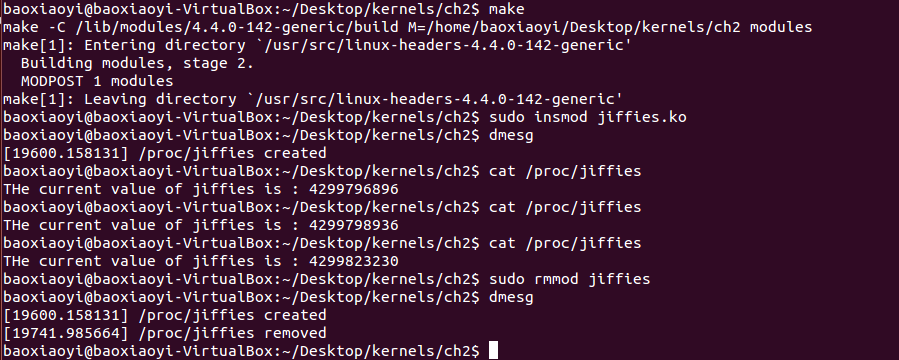
\includegraphics[scale=0.8]{res1.png}
        \caption{Result for assignment 1}
        \label{fig:fig1}
    \end{figure}
   
 \newpage
 
    \begin{figure}[h!]
        \centering
        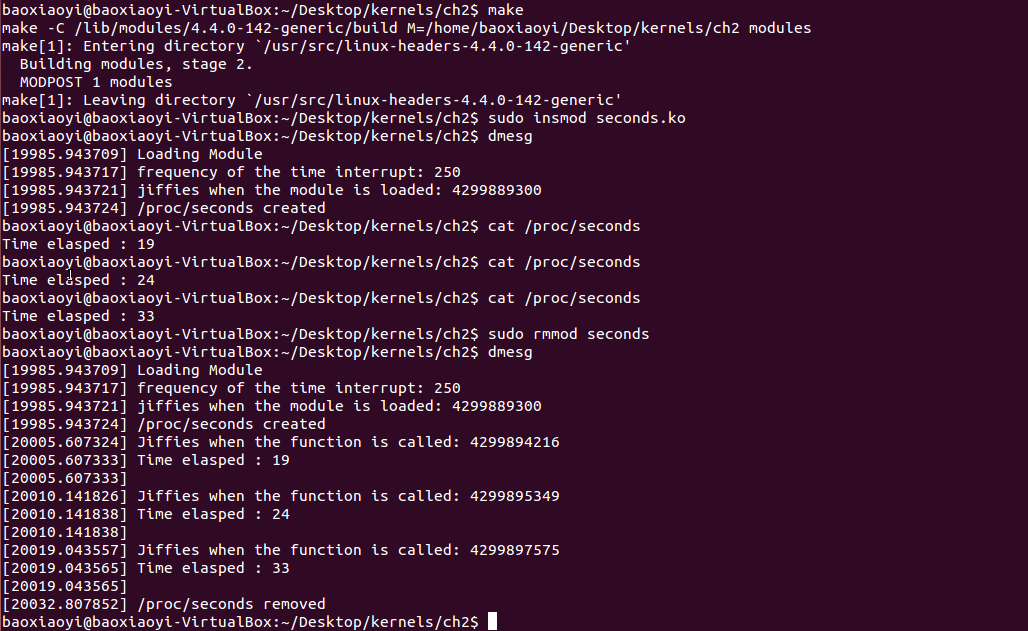
\includegraphics[scale=0.8]{res2.png}
        \caption{Result for assignment 2}
        \label{fig:fig2}
    \end{figure}

\section{Future work}
It is just the start of our exploration into operating system, and of course there are a lot more to be done. To be more specific, there are two points that we may improve in the future:
\begin{itemize}
    \item Elapsed time as a floating number. Thereby, the description of elapsed time can be more precise to users.
    \item A pointer for passing the value of jiffies when the module is loaded. 
\end{itemize}
\newpage


\end{document}
